\section{Compatibility Testing} \label{compatibility_testing}\label{sec:compatibility}
For the credential swapping method to work correctly, the dummy credentials must be visible in the outgoing request traffic.  Client scripts could alter the values entered for the username and password in ways that would disrupt recognition. In this section, we describe the \SwapScan\ tool we built to perform compatibility testing (Section~\ref{swap_scan}), reports on how we tested Alexa's top million websites (Section~\ref{sec:scanning}), and present our compatibility results (Section \ref{finding_dummy_credentials}).  \SwapScan\ uses heuristics to find login forms on web sites, and then automates the login process using the dummy username and password. For sites where a test login can be performed, \SwapScan\ checks the request traffic for the dummy username and password strings. We found this test to be successful on 98\% of the tested logins, which gives us a high confidence that \SecPass\ would work on a majority of the web. As a by-product of our compatibility test, we also found many insecure login form development practices, which are not directly relevant to password managers; we report on these findings in Appendix~\ref{extracting_other_information}. 
%\dnote{worth mentioning other results that are byproduct of these tests?}
%\dnote{add forward section references to this paragraph}


%The purpose of the scan was to test whether a majority of websites would be compatible with \SecPass's credentials-swapping feature. This results section is divided as follows: Finding the dummy credentials in traffic (Section \ref{finding_dummy_credentials}), Extracting other information from the login requests (\ref{extracting_other_information}), and Reasons why some sites' login were not tested (\ref{reasons_for_failures}). 

%\SwapScan, our login automation tool, builds upon the code and ideas of two works: OpenWPM~\cite{englehardt2016census} and SSOScan~\cite{Zhou2014}. 

%\dnote{I updated the figure - the only (intentional!) substantive change is what happens after "No" from the "Dummy credentials detected?" box.  Before, it looked like it went back to $C_A$, but I don't think this makes sense. Please confirm that what I did makes sense now. May be missing another state needs for if any network traffic is detected that is classified differently?}
%\hnote{I think the figure looks good. Details of the network traffic is analyzed afterwards, so they don't belong in the state diagram.}
\iffalse
\begin{figure*}
\centering
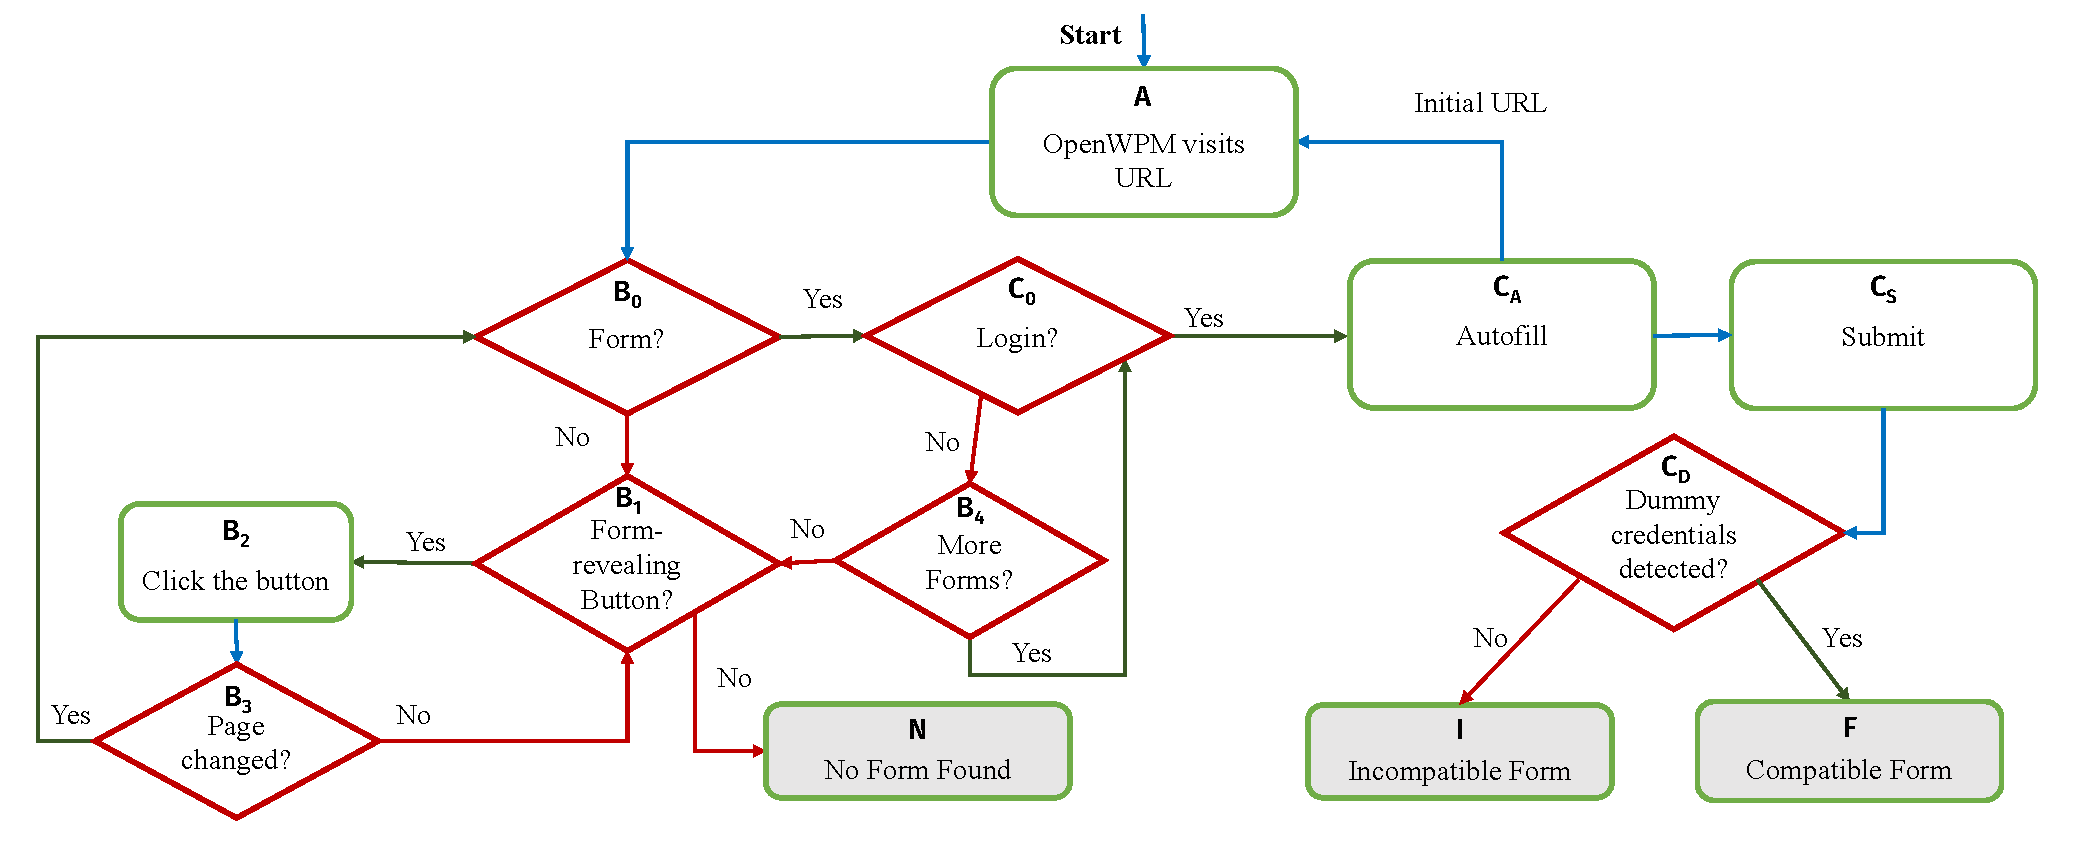
\includegraphics[width=0.8\textwidth]{authscanfigure.pdf}
\caption{State diagram of \SwapScan\ }
\label{SwapScan_diagram}
\end{figure*}
\fi
\subsection{\SwapScan} \label{swap_scan}

\SwapScan, our login automation tool, is built on top of OpenWPM, a fully-automated, open-source framework for large-scale web scanning~\cite{englehardt2016census}. OpenWMP provides scalability by wrapping Selenium instances in a driver that monitors their activity, ensuring that if the web page stalls or if one Selenium crashes, the test would continue. OpenWPM, which was originally intended to measure web privacy from third-party scripts, also includes a proxy and a series of hooks for data collection --- two features that were essential for our experiments. 

\SwapScan\ starts by using OpenWPM to visit a URL from a list of URLs of the front page of websites, and then uses heuristics to scan the site to attempt to find, fill in, and submit a login form. Our approach is adapted from SSOScan~\cite{Zhou2014}, but is more complicated since we are looking for login forms instead of SSO buttons. 
% Another difference is that there is an easily-recognized HTTP response from Facebook if you have clicked on the correct button, whereas we would only know that we clicked on the correct button and tried the right form if we eventually see request traffic containing our dummy credential strings. To overcome this challenge, \SwapScan\ has a more sophisticated scan state interpreter and fine-grained control over how web pages are rechecked.

 %To avoid repeat work, each possible form or form-revealing button is only tried exactly once \dnote{do you mean to say each is tried exactly once, or they are all tried at most once?}.
 
\shortsection{Finding Login Forms} After visiting the URL, \SwapScan\ attempts to find a login form on the website. 
The strongest indicator of a potential authentication form is the presence of a HTML element with \keyword{type=password} in the form children. Once an authentication form is found, \SwapScan\ determines whether the current form is for login or registration. If there are two password children in the form, then the form is likely a registration form. Other indicators used to separate registration forms from logins include keywords in the title of the page, keywords in the form attributes, and whether the form contains an input with registration topics (e.g., birthdate, security question). \SwapScan\ determines the topic of an input box by matching regexes with element attribute values.  If the candidate form is not a login, \SwapScan\ will try other forms on the page.

%\dnote{wasn't the "Heuristics" section mostly about "Revealing the login form"?  Can this be organized to better fit the actual search process?  Probably best not to have any Heuristics shortsection, and instead just have shortsections on "Revealing Candidate Login Forms" and "Recognizing and Submitting Login Forms" ?}

% \shortsection{Recognizing Login Forms} \label{find_login} 
If no suitable form is found on the current page, \SwapScan\ uses heuristics to click on buttons likely to reveal forms until it finds one or reaches the maximum number of attempts allowed. Candidate login-revealing buttons are chosen from the page and ranked by matching regular expressions such as \code{[Ll][Oo][Gg][liOo][Nn]} with each of the attribute values or the innerHTML of a \textit{visible} node~\cite{Zhou2014}. The likely candidates are ranked by the frequency of the matched regular expressions and the attribute the keywords are found in (e.g., the \keyword{innerText} of an element would be a better indicator of the purpose of the login).  Invisible elements are not considered because a human user would not interact with them, and single-sign-on buttons are ruled out completely. If none of the attempts lead to a login form, \SwapScan\ decides "No Login Found", concluding this test.

\shortsection{Testing Submission} If a login form is found, it is autofilled with the dummy username and password and submitted.  Outgoing traffic is observer to look for the dummy username and password.  \SwapScan\ also saves all outgoing traffic from the browser for analysis explained in Section~\ref{sec:scanning}.   

%After simulating a real login process by pressing the "submit" button, \SwapScan\ intercepts the traffic for the dummy credential strings, stopping the test on the current site if those strings are present. If not, \SwapScan\ goes back to the front page and tries a different set of buttons. 

%\shortsection{Heuristics} \label{heuristics} The form-revealing buttons, forms, and input fields are interpreted by matching regular expressions such as \code{[Ll][Oo][Gg][liOo][Nn]} with each of the attribute values or the innerHTML of a \textit{visible} node~\cite{Zhou2014}. Invisible elements are not considered because a human user would not interact with them. 
%\dnote{need a bit of set-up here - are you assigning a score to every element, sorting them by that score, and then trying the top K?}
%The element priority, whether it is a form or form-revealing button to try, is ranked based on the number of occurrences of relevant regular expressions. Those with attributes containing keywords for single-sign-on, such as "Facebook", "Google" or "Twitter" suffer immense deduction of points and priority if we are not currently on the social media website. \dnote{previous sentence too confusing for me to parse - is having SSO on a form a positive or negative signal?}Buttons, links, or forms with attributes hinting at registration are ruled out completely. 

%Once a \dnote{what? conjectured form-revealing link?} is located, \SecPass\ scanner clicks on the most likely candidate and repeats the process outlined above, checking for the presence of a login form in the resulting response page. As a result, we could only locate a form if its id, for example, matches the regular expression above.  \dnote{I'm more confused by this than I should be - does this section map to something in Figure 3?  Can the two kinds of heuristics be separated:
%1. finding form-revealing buttons
%2. determining if an element is a login-form}

 % \dnote{this is about testing if something is a login form - clearer to separate into those steps}



%\shortsection{Architectural Choices} There are several tools capable of simulating human interaction with the web: PhantomJS~\cite{PhantomJS}, browser add-on drivers (e.g. Firefox Add-on SDK~\cite{FirefoxSDK}), and Selenium~\cite{Selenium}. Fast and relatively simple, PhantomJS is a headless WebKit supporting a JavaScript API that could be used to access and manipulate the DOM of the page. However, it lacks many of the capabilities of the real browser and does not load all third-party traffic. Browser add-on drivers, while powerful, are not made for lengthy operations and suffer from memory leaks. For example, the Firefox add-on driver can only open around 800 websites before crashing and breaks when subjected to frequent reboots. While slow compared to PhantomJS and browser add-on drivers, Selenium proved to be the best option for this task, though it also has its weaknesses. Selenium is not designed to automate many different websites, but rather to test a website for a developer who starts the test knowing the identification of every node on the webpage. However, it does have a wide range of APIs that makes it easier to interact with the DOM than writing raw JavaScript. 




%\dnote{does a description of OpenWPM belong here alos?} 


%If the unique strings are not found in the traffic, the website is flagged down for a closer look at its login process. 

\subsection{Scanning} \label{sec:scanning}


%\begin{figure*}
%\centering
%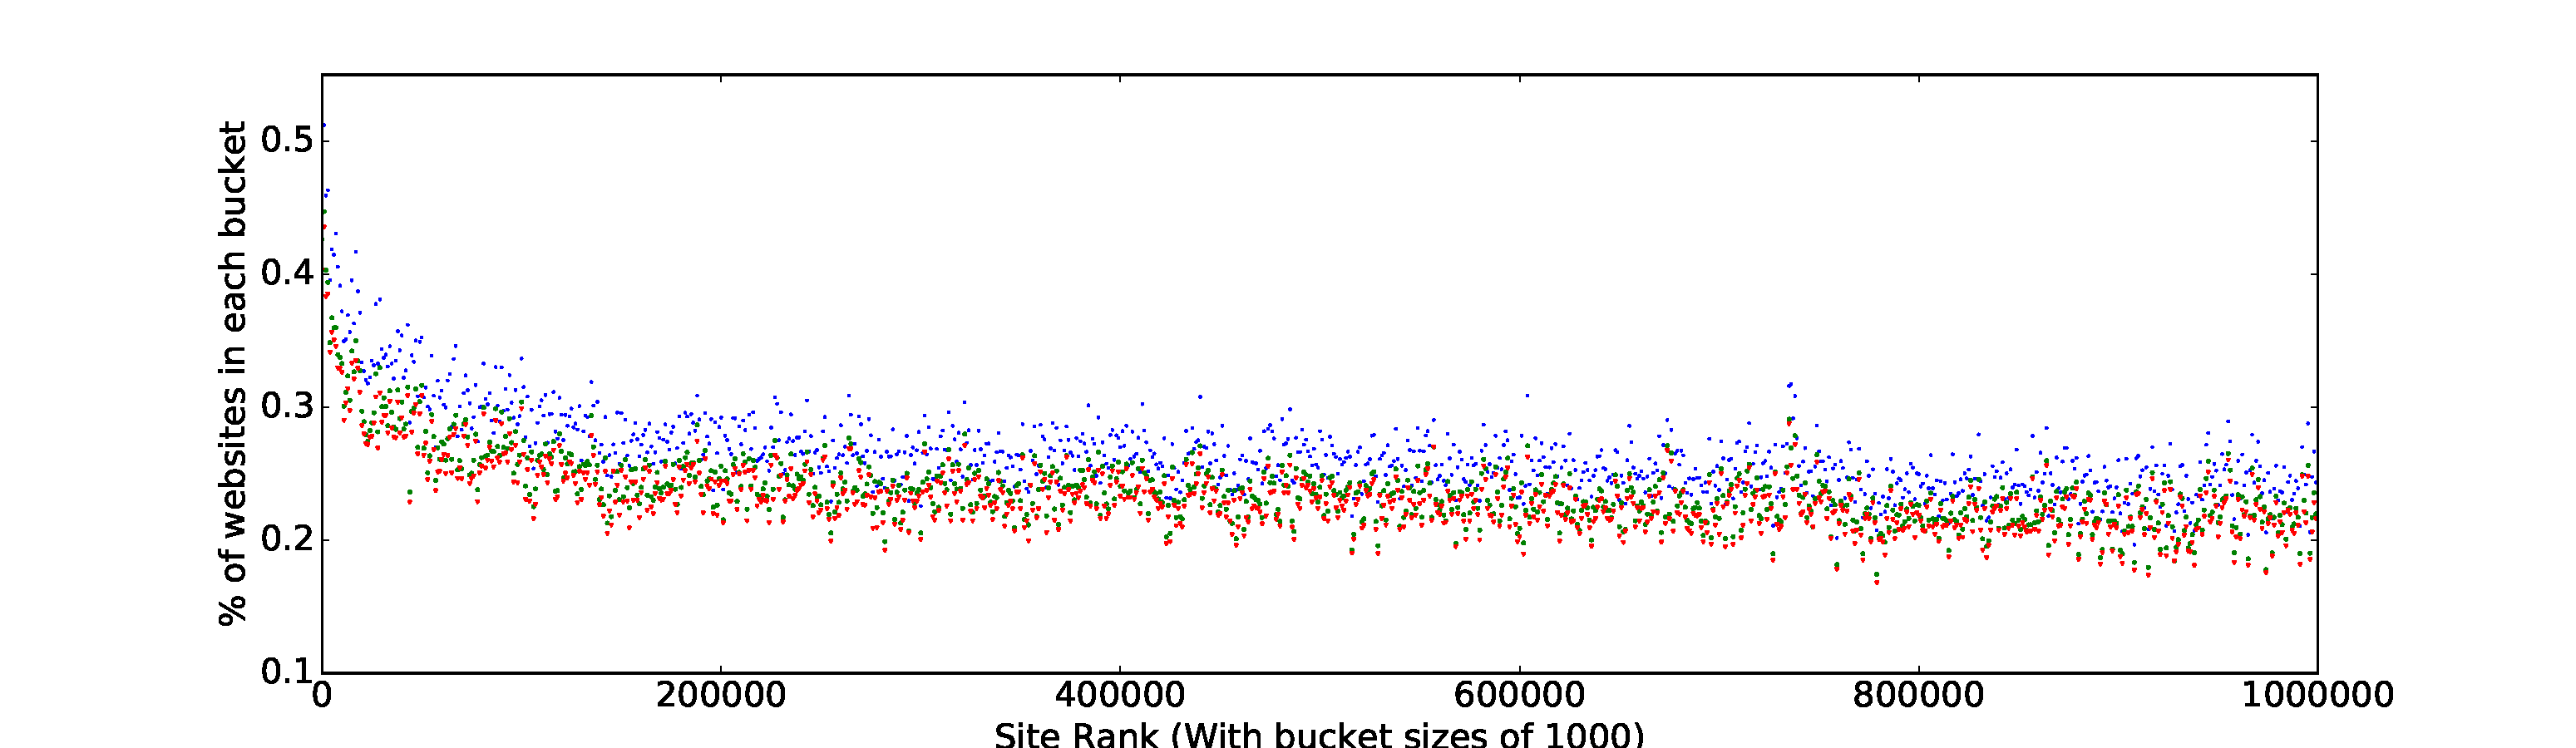
\includegraphics[width=\linewidth]{scan_overview_graph.pdf}
%\caption{Overview of scan results. This is difficult to see, so I think we should just include the graph above this one. The blue shows percent of sites login was found, the green shows the percent of sites where login was successfully submitted, and the red shows the percent of websites where we saw the credentials.}
%\label{percent_login_found}
%\end{figure*}

In February 2017, we used \SwapScan\ to scan Alexa's top million websites. 
This took approximately 16 hours using 200 Amazon AWS c4.2large instances, each running 10 parallel scans, averaging around 2 minutes per website. 


%\dnote{in the tests, are these unique long strings that never appear otherwise in the traffic?  will you also look for the MD5's of those strings?}



%Out of the 14214 websites whose front page loaded within the allotted time, \SwapScan\ found that 5527 (39\%) of the websites had a form that had indications of a login form. \SwapScan\ autofilled the form  and attempted to submit the form via {\tt{Element.submit()}}, during which 5248 (95\%) of the found forms returned statuses of submission success. Out of the forms that were successfully submitted, 4867 (93\%) of the submissions yielded traffic during the 3 seconds that \SwapScan\ waited for a response from the page.

%All the traffic up to 3 seconds after the submission were collected and analyzed. Out of the number of sites whose login form initiated outgoing traffic, \SwapScan\ detected 4710 (97\%) sites with both username and password dummy strings, 98 ($<$2\%) sites with username only string, and 28 ($<$1\%) sites with password only strings in the request. 


%\subsection{Scan Results} \label{scan_results}

Figures~\ref{scan_success} and \ref{percent_login_found} summarize the results of the scan.  The key finding, discussed in Section~\ref{finding_dummy_credentials}, is that the password swapping approach works on the vast majority of websites (98\% in our study).  Here, we explain why some websites were not tested and the success rate for finding login forms among those that were tested.

\begin{figure}[bt]
\centering
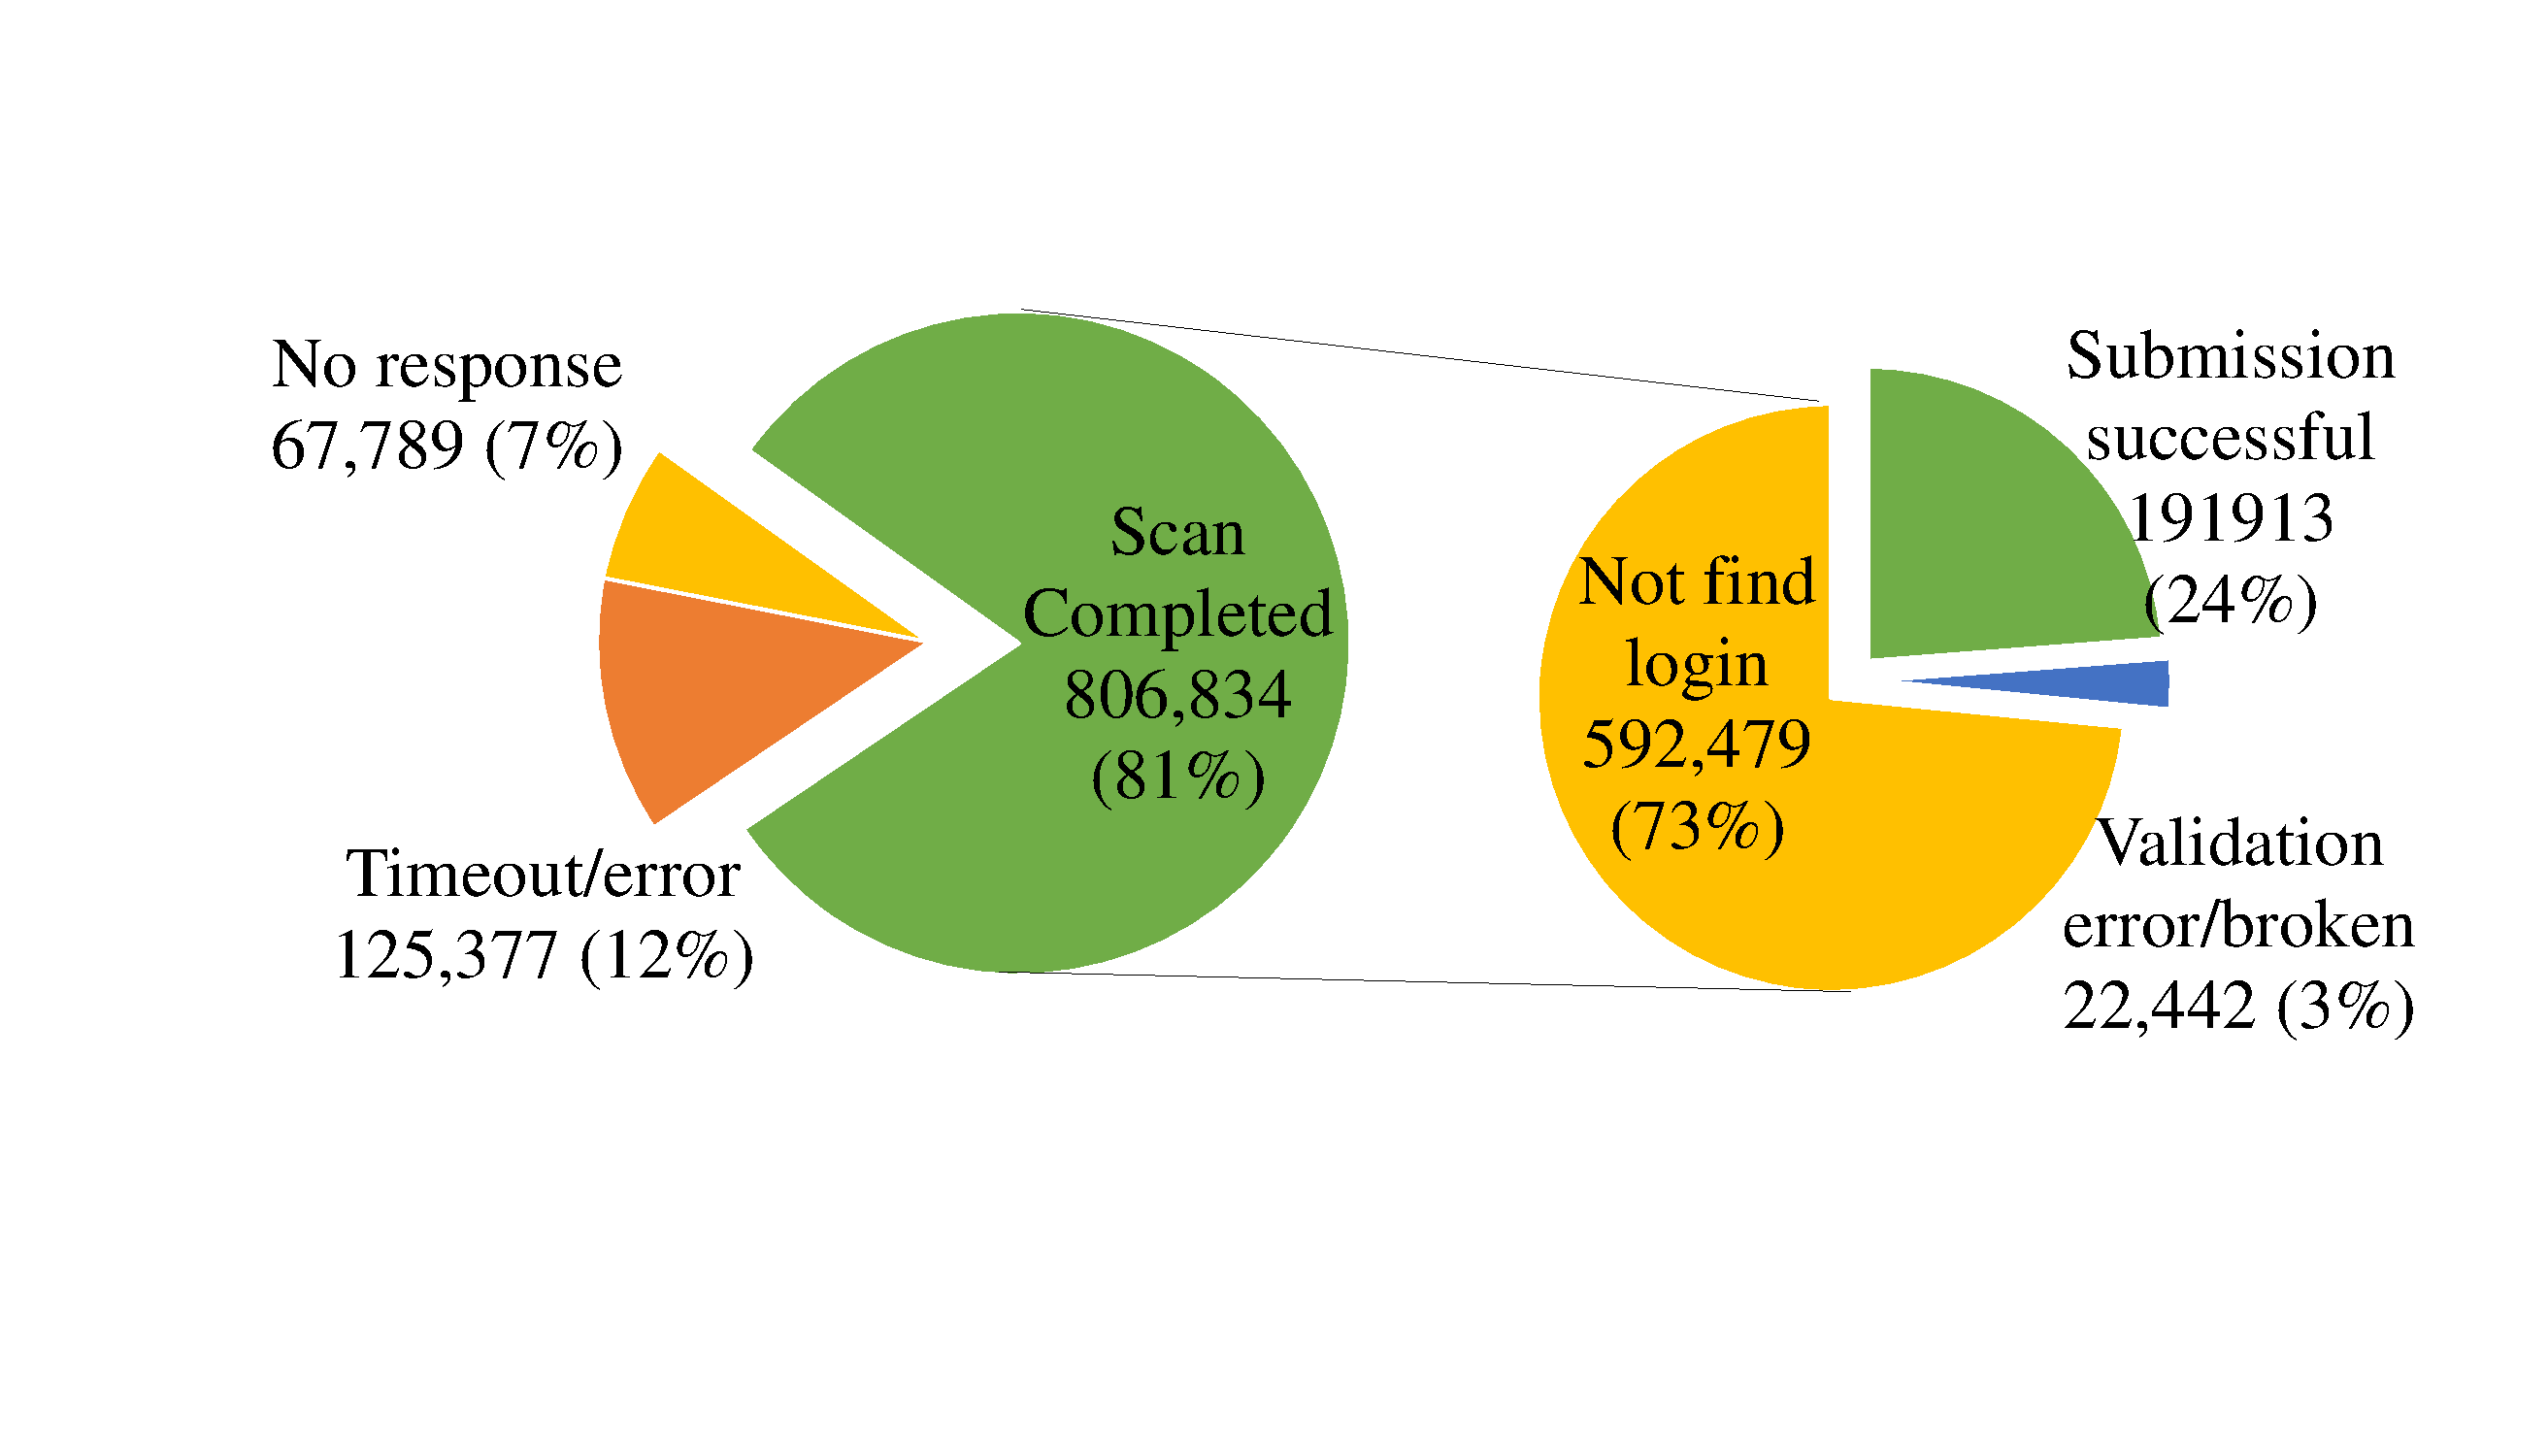
\includegraphics[width=0.95\linewidth]{scan_success.pdf}
\caption{Overview of scan results}
\label{scan_success}
\end{figure}

\begin{figure}[bt]
\centering
\includegraphics[width=\linewidth]{percent_login_found.pdf}
\caption{Percent of sites where login is found by popularity rank. {\rm Each bucket is for 1000 sites for which the scan completed.}}
\label{percent_login_found}
\end{figure}

\shortsection{Nonresponsive Websites} Out of the 1 million sites attempted, 932,211 (93\%) responded with 2xx or 3xx response codes. This result is consistent with OpenWPM's scan result in January 2016, which found that 917,261 (92\%) of the websites successfully loaded~\cite{englehardt2016census} 

The scanner imposes a four-minute timeout for the total time to scan each website. Time outs and errors are affected by network speed and slow server response times (this primarily impacts websites hosted in other countries). \SwapScan\ considers the scan incomplete if it has not completed the full scan itinerary at a maximum depth before the allotted four minutes expire. Errors and timeouts excluded 123,481 (12\%) of the websites out from the scan. 


%are mostly due to international websites that load third-party scripts slowly. Sometimes, the page never finishes loading the scripts. \SwapScan\ waits for all the scripts on the page to finish loading before starting the scan, as login forms behavior can sometimes be affected by script behavior. Another factor that slows tests down is finding login-revealing buttons. If the website has an extraordinarily large number of elements on the page and the login-revealing button isn't located on the top of the page, then it may take a while to go through every element's attributes checking for regexes. 

%Errors occur when the page changes unpredictably or a connection error occurs during a scan of a website.  

\shortsection{No Discovered Login Forms} Among the remaining 806,834 sites, \SwapScan\ found 214,355 (27\%) websites with native login forms. Some sites do not provide any native login form, either because they do not have user accounts or only support single-sign-on authentication, which we do not include since there is no password to manage.  
There are several possible reasons, however, why \SwapScan\ could fail to find a login form on a site that has one.  The scanning heuristics assume login forms always include an element with \keyword{type=password}, but this does not hold for all login forms. For example, some sites use a two-step login process where the username is collected by the first form, and the password input is only revealed after the visitor submits a username.
Our heuristics only consider English-language keywords, so may miss login forms labeled with other languages. Finally, we assume that an important login form would be accessible within a few clicks from the front page of a website. 

Figure~\ref{percent_login_found} shows the fraction of websites for which a login was found as the popularity of the site decreases.  The success rate reflects the likelihood that more popular sites are more likely to provide user accounts, less likely to rely fully on single-sign-on authentication, and perhaps more likely to be designed in a way that makes the login form easier for an automated scanner to find. We are not able to distinguish among these (and other) possible reasons in our study, however.

Out of the 214,355 sites found with native logins, 22,442 (10\%) sites' login did not respond with an outbound request upon submission. This may be due to broken logins or client-side validation errors.  The remaining 191,913 sites (90\%) were tested for compatibility with \SecPass, and these are the sites analyzed in Section~\ref{finding_dummy_credentials}.

\shortsection{Comparison with Previous Results} The largest previous scan of website login forms %\dnote{is this true?} \hnote{looks like it}
was Acker et al.'s 2017 study of the top 100,000 websites~\cite{acker2017}. They reported finding 48,547 logins on those sites, where our scan only found 25,449. There are several 
reasons for the difference.  We used heuristics to eliminate registration forms, ruling out forms with any indications of a registration-related input.  Their scan counted any form with a \keyword{type=password} field as a login form, so counted some forms that were not considered login forms by our scan. Acker et al.\ counted 2,760 as not reachable within the 51\% failed websites, while we considered 16,584 websites as not having completed the scan because they were either broken or did not respond fast enough to make our 4 minute threshold. Our scan required more interactions with the websites because we needed to observe the actual submission traffic, not just find the form, so more websites timed out. %\dnote{? is this the reason?  I'm not sure I really understood the timeout sentence before this one}
Further, we relied on the fact that the website was functioning quickly enough and that the login was reachable from the front page, whereas Acker et al.'s use of crawlers and search engines may have revealed login forms that were not directly accessible from the front page, which boosted their rate of finding logins.\footnote{We considered using search queries for our scan also, but decided against this because of the unavailability of search engine APIs that allow enough queries for the larger scale of our scan.} 
%\dnote{added this note, unless its mentioned elsewhere. if you can add some details to the footnote, please do}

%\dnote{I moved this down here, but may belong above. Not clear to me if you are counting these in your rates or not (and if Acker+ is counting them the same way)}

%\shortsection{Login forms not successfully submitted}

%\SwapScan\ attempted to submit every login form that it found. A submission is considered a success only when the submission yielded traffic up to 3 seconds following the event. Reasons why some submission failed include changed page, broken form, and client-side validation blocking. 

\iffalse
\begin{figure}[tb]
\centering
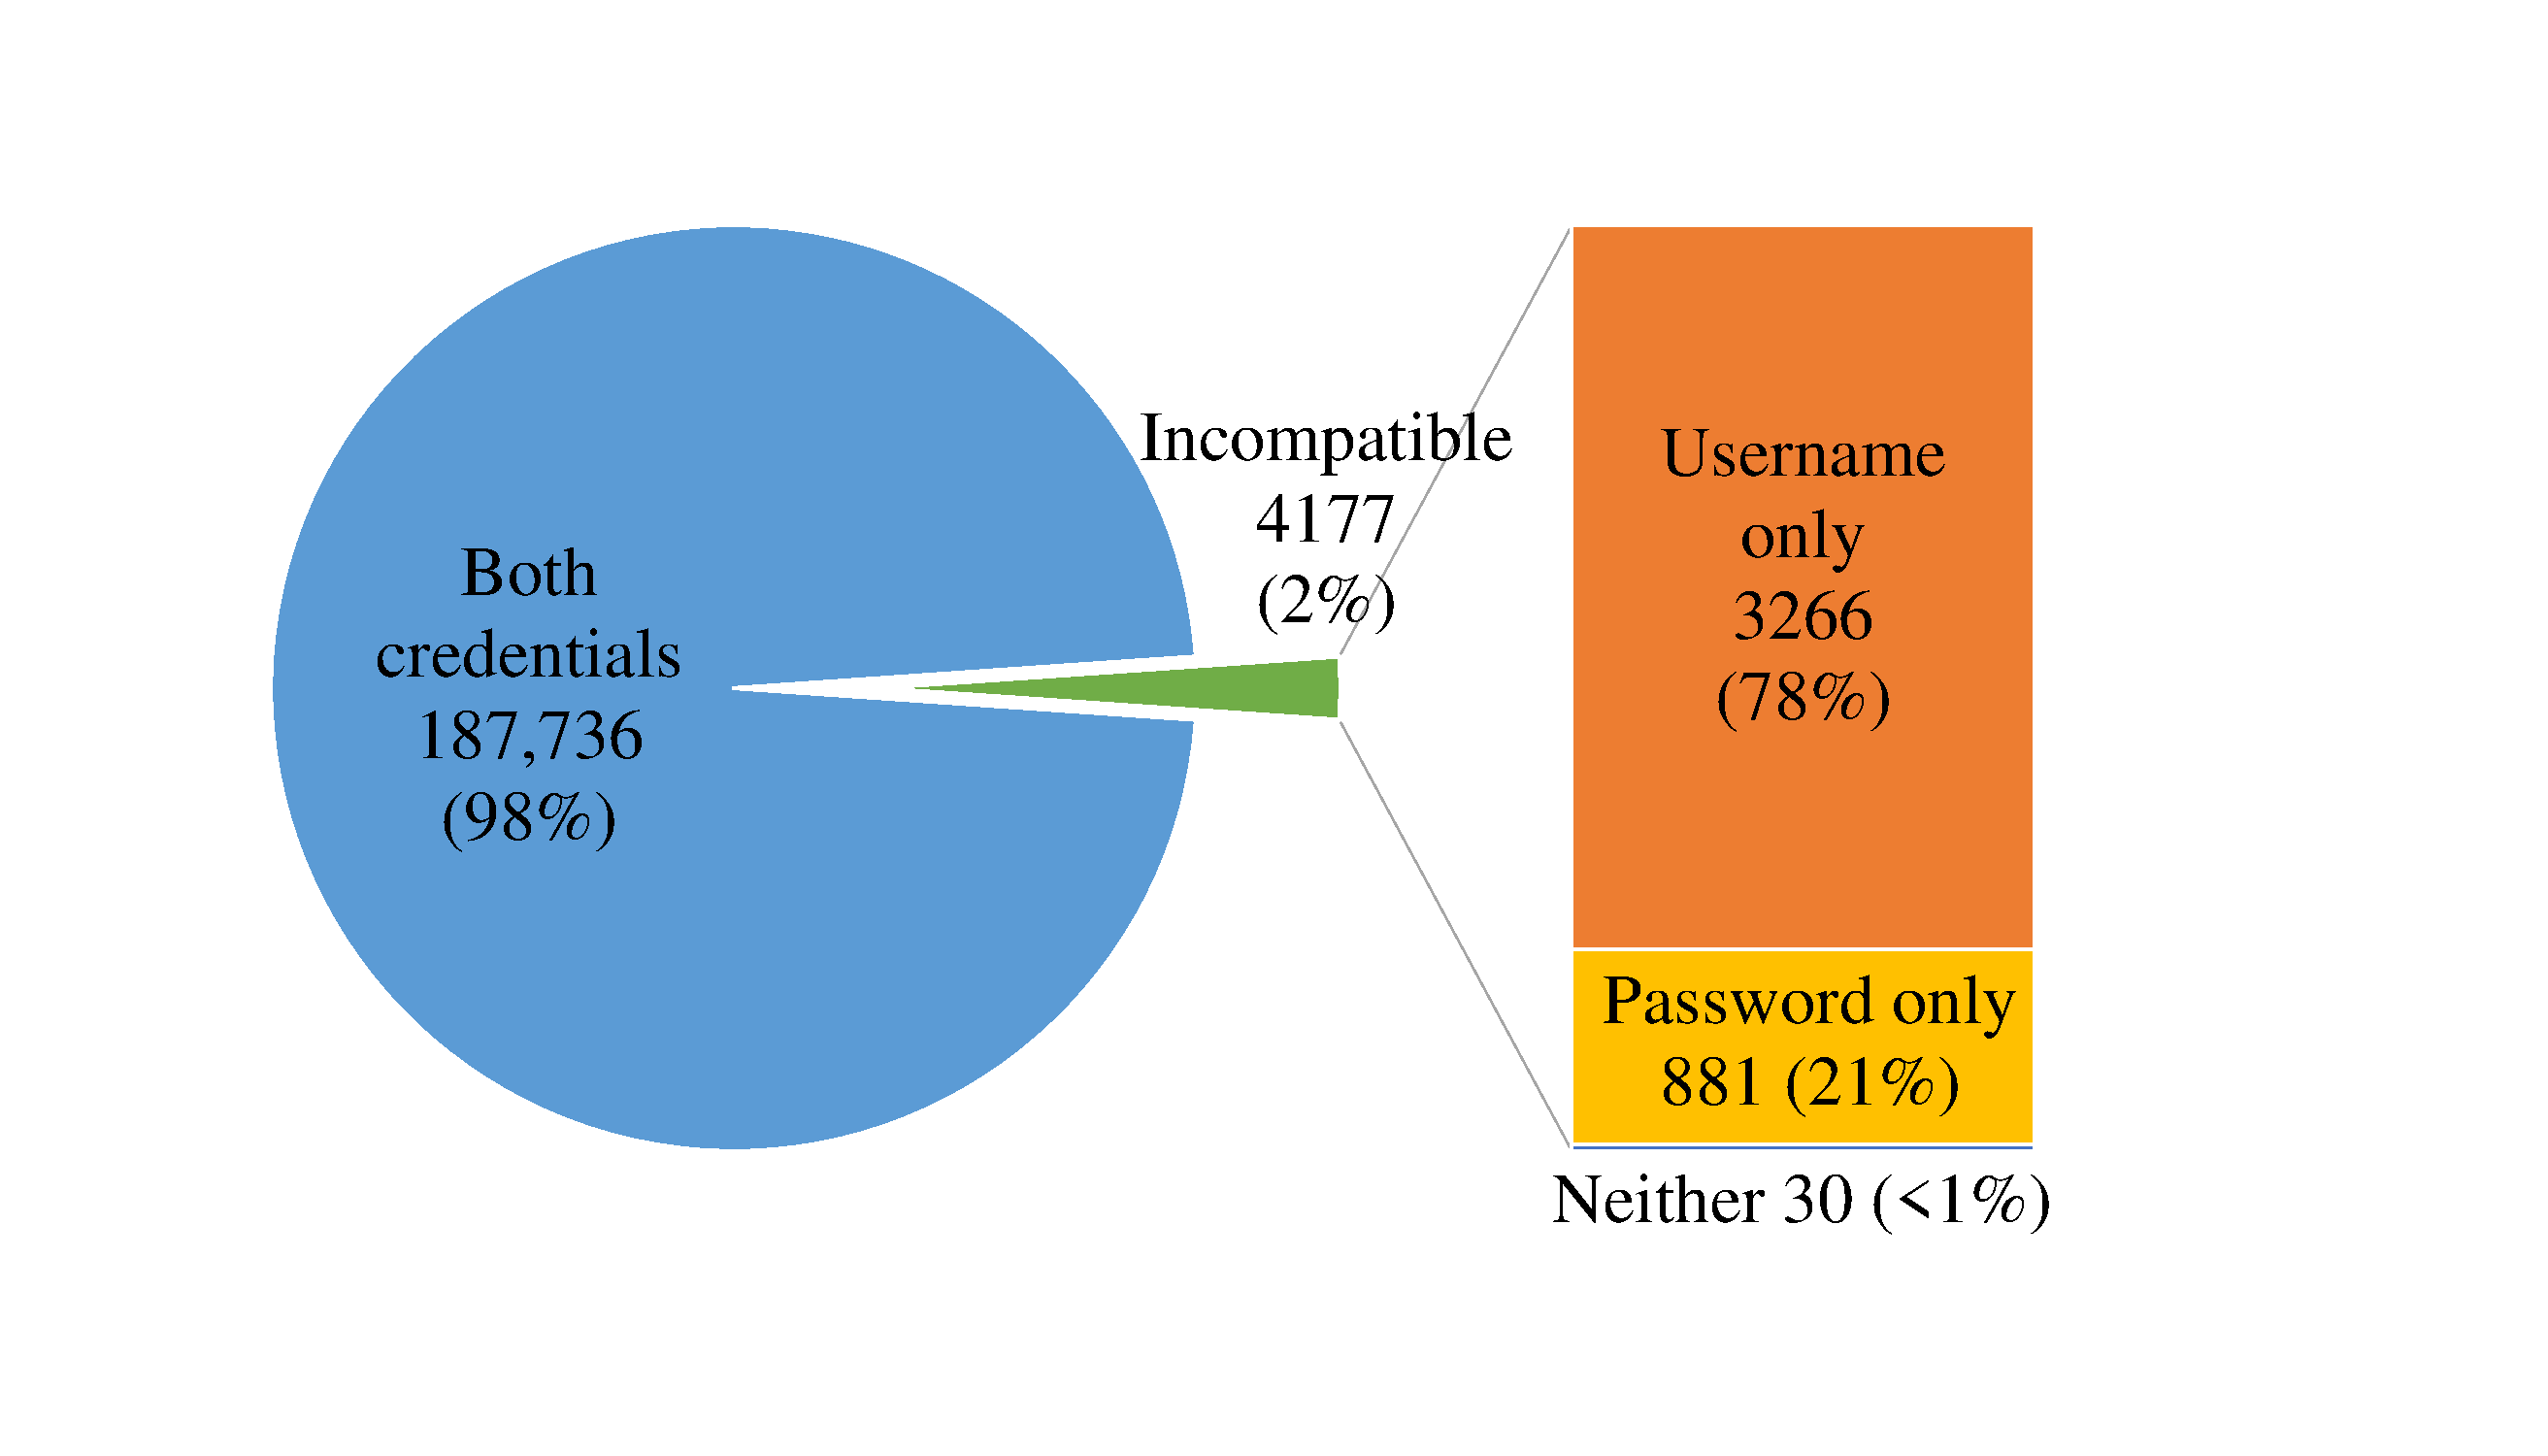
\includegraphics[width=0.8\linewidth]{compatibility.pdf}
\caption{Dummy credentials detected in traffic}
\label{credentials_breakdown}
\end{figure}
\fi 

\subsection{Compatibility Results} \label{finding_dummy_credentials}

A site is counted as compatible if both the username and password dummy credentials are recognized in any request. \SwapScan\ records all network traffic during a 3-second duration following a form submission. Of the websites where forms that were successfully found and submitted, 187,736 (98\%) appeared to be compatible. On these sites, both the dummy username and password were observed in the intercepted traffic so the credential substitution approach should work. Note that while we define compatibility broadly, for security reasons our \SecPass\ password manager only reveals real credentials in HTTPS POST requests to the correct target domain (Section~\ref{sec:client_side_security_analysis}). %\hnote{edited}  good

In cases where multiple requests are sent following a login form submission, we consider the request that contained the most information (e.g., we would favor a request containing both username and password over a request only containing the username). When we only see one of the username or the password in a request, we would check other requests from that website to see if the missing credential is in a different request.

We found some websites that were doing client-side encryption on credentials before sending them out to the server. We found 817 ($<$1\%) of websites sending their requests out with a plaintext username and MD5-hashed password. These websites are counted as compatibale because \SecPass\ can look for the MD5-hashed dummy password in outgoing traffic and replace it with the MD5-hash of the real password.

\shortsection{Reasons for Incompatibility}
Of the tested sites, 4177 (2\%) appear to be incompatible with credential substitution.   %As summarized in Figure~\ref{credentials_breakdown},
For 3266 (78\%) of these, the dummy username was observed in intercepted traffic but not the dummy password. We manually examined a sample of ten of these sites, and found that nine of them were sending the dummy password transformed by some function other than MD5 hash.  The remaining sampled site had an empty password field, which means that the site was either broken or did not send the password because client-side validation failed. The (probably misguided) inclination for sites to do client-side hashing of passwords explains why not observing the dummy password is the most common reason for incompatibility.  

We also manually examined a sample of ten sites selected from the 881 incompatible sites where the password was observed but not the username.  Three of these sent requests with empty username fields, one with a transformed username (but not a cryptographic hash).  For the six remaining sites, we could not determine the reason why the dummy username had not appeared in the traffic.

%dnote{I'm not exactly sure what to do with this unusual requests section - parts of it are explaining reasons for incompatibility (I think), and other parts seem like they belong in the "Other Results" section?}
%\shortsection{Unusual Requests} Though the majority of these websites sent the credentials using conventional means of putting the credentials in the content of POST requests, we found some using insecure practices. While it is conventional and safer to use POST requests to send login credentials to the server, 4489 (2.4\%) of the tested logins still used GET requests and 30 ($<$0.2\%) of the websites used another method to send their credentials. 

%While manually examining login requests that put the username and password in different requests or separate sections of a request, we found that 2 sites put the username and password in separate header fields, 7 sites put username and password in different requests, and 13 put the username in the request URL but the password in the request content. 

%Some sites cut off the username and/or password strings at as few as 4 characters long. We do not consider partial dummy credentials that are less than 6 characters long, and they counted in the 2\% incompatible (neither category in Figure~\ref{credentials_breakdown}) category. %\dnote{failed = incompatible? here? - are these in the 30 neither in Fig 4?}

One threat to validity is searching for dummy credentials that are not unique and long. We choose credentials with a goal of passing any client-side validation checks, so they could not be long random strings. Still, there is little risk of encountering the same string meant for another context, as our checking scope is limited to requests made in response to our form submissions. 

\SwapScan\ found that the password swapping would work on the preponderance (98\%) of websites in the top million, and could be successfully deployed in a modern browser to work on today's web. If any popular sites are incompatible (i.e. \url{www.sohu.com}) %\dnote{what was the most popular ranked site that was incompatible?}
, it may be necessary to include special rules for matching custom client-side password transformations. At worst, users can fall back to manual logins for incompatible sites.


